
\section{第~6~章的练习}
\label{sec:ch14-exercises-ch6}

\begin{exercise}\label{ex:ch14-022-torus-translation}
验证：映射
\[
\begin{array}{rcl}
\RR^2 & \longrightarrow & \RR^2\\
(p,q) & \longmapsto & (p,q+1/2)
\end{array}
\]
在\trTorus{} $T^2=\RR^2/\ZZ^2$ 上导出的商映射，是一个保持\trSymplecticForm{}（$\varphi^\star\omega=\omega$）的\trDiffeomorphism{} $\varphi$，但它没有任何\trFixedPoint。证明：在 $T^2$ 上存在一个\trVectorField{} $X$，使得
\[
\varphi=\varphi_X^1\text{，}
\]
但 $X$ 不是一个\trHamiltonian\trVectorField。
\end{exercise}

\begin{exercise}\label{ex:ch14-023-circle-action-fixed-points}
设 $W$ 是一个\trSymplectic\trManifold，配有保持\trSymplecticForm{}的一个圆作用。假设 $W$ 是\trSimplyConnected{}的。证明：这个作用与一个\trPeriodic\trHamiltonian{}量 $H\colon W\to\RR$ 相伴随（按\cref{ex:ch14-018-periodic-hamiltonian}的意义）。设 $\zeta\in S^1$，并设 $\varphi$ 是由 $\varphi(x)=\zeta\cdot x$ 定义的\trDiffeomorphism。证明：$\varphi$ 是一个\trHamiltonian\trDiffeomorphism，并且它至少有
\[
\sum_i\dim HM_i(W;\ZZ/2)
\]
个\trFixedPoint。\footnote{译注：本练习照原书排印，惟末一断言须以 $W$ \trCompact{}（或诸\trTrajectory{}相对紧）为前提，非紧时它可以不成立：例如取 $W=\CC^2\setminus\{0\}$（\trSimplyConnected{}），配上保持 $\omega$ 的\trHopf{}圆作用，则对 $\zeta\neq1$，$\varphi(x)=\zeta\cdot x$ 没有任何\trFixedPoint，而 $HM_*(W;\ZZ/2)\cong H_*(S^3;\ZZ/2)$ 只有一项非零（其和为 $1$）。故应补 $W$ \trCompact{}（或诸\trTrajectory{}相对紧）之条件；此处照原书排印，存疑备案。——译者注}
\end{exercise}

\begin{exercise}\label{ex:ch14-024-loop-space-derivation}
设 $x\in\scr{L}W$，并设 $u$ 是 $\scr{L}W$ 中经过 $x$ 的一条曲线，也就是说，一个映射
\[
u\colon\RR\times S^1\longrightarrow W
\]
满足 $u(0,t)=x(t)$。设 $Y$ 是由 $u$ 定义的、切于 $\scr{L}W$ 的那个向量。对于函数 $f\colon\scr{L}W\to\RR$，我们令
\[
Y(x)\cdot f=\frac{\partial}{\partial s}\,f\circ u(s,t)\big|_{s=0}\text{。}
\]
证明：这个公式确实定义了某个东西，而且这个东西在这些函数上是一个\textbf{\trDerivation}（derivation）。
\end{exercise}

\begin{exercise}\label{ex:ch14-025-torus-hamiltonians}
在\trTorus{} $\mathbf{T}^2=\RR/\ZZ\times\RR/\ZZ$ 上，我们考虑\trSymplecticForm{} $\omega=dy\wedge dx$。设 $H$ 与 $K$ 是从 $\RR^2$ 到 $\RR$ 的由
\[
H(x,y)=\frac{1}{2\pi}\cos(2\pi x)\text{，}\qquad
K(x,y)=\frac{1}{2\pi}\sin(2\pi y)
\]
定义的函数。证明：$H$ 与 $K$ 在 $\mathbf{T}^2$ 上定义了（\trAutonomous{}的）\trHamiltonian{}量，并求出与之相伴随的\trHamiltonian\trVectorField{} $X_H$ 与 $X_K$。\footnote{译注：原书此处印作“$H_K$”；按上下文系与 $X_H$ 并列的、$K$ 所对应的\trHamiltonian\trVectorField，疑应为 $X_K$；此处径改。——译者注}

求出 $X_H$ 的\trFlow{} $\varphi_t$ 与 $X_K$ 的\trFlow{} $\psi_t$，以及 $X_H$ 与 $X_K$ 的以 1 为\trPeriodic{}的诸\trPeriodic\trTrajectory。$H$ 与 $K$ 这两个\trHamiltonian{}量是否\trNondegenerate{}？

计算复合 $\sigma_t=\psi_t\circ\varphi_t$。求出生成\trHamiltonian\trIsotopy{} $\sigma_t$ 的\trHamiltonian{}量 $F_t$（参见\cref{ex:ch14-007-hamiltonian-diffeomorphism-group}）。求出 $X_{F_t}$ 的以 1 为\trPeriodic{}的诸\trPeriodic\trTrajectory，并指出其中哪些是\trContractible{}的。证明：$F_t$ 是\trNondegenerate{}的。\footnote{译注：本练习照原书排印，惟末段有两点须留意。其一，按\cref{ex:ch14-007-hamiltonian-diffeomorphism-group}(1)，生成 $\sigma_t=\psi_t\circ\varphi_t$ 的是 $F_t=K+H\circ\psi_t^{-1}$，而它一般并不以 $1$ 为\trPeriodic（$F_{t+1}-F_t$ 并非只含 $t$）；要谈论“$X_{F_t}$ 的以 1 为\trPeriodic{}的诸\trPeriodic\trTrajectory”，须先把 $F_t$ 沿 $t$ 作\trPeriodic{}延拓（例如经端点的重新\trParametrization），且 $\sigma_1=\psi_1\circ\varphi_1$ 的诸\trFixedPoint{}所对应的闭区间 $[0,1]$ \trTrajectory{}与延拓后的整\trPeriodic{}解亦须加以区分。其二，$\sigma_1$ 共有 $16$ 个\trFixedPoint，其中仅 $4$ 个\trNondegenerate，而这 $4$ 个恰为常值\trTrajectory（故\trContractible{}），其余 $12$ 个皆\trDegenerate{}且不\trContractible——故“$F_t$ 是\trNondegenerate{}的”只在\trContractible\trTrajectory{}一类上成立。此处照原书排印，存疑备案。——译者注}
\end{exercise}

\begin{exercise}\label{ex:ch14-026-action-form-closed}
在空间 $\scr{L}W$ 上，考虑\trActionForm
\[
(\alpha_H)_x(Y)=\int_0^1\omega(\dot{x}(t)-X_t(x(t)),Y(t))\,dt\text{。}
\]
设 $x_0\in\scr{L}W$ 是一个取定的\trLoop。我们取定 $x_0$ 到\trDisk{} $D^2$ 的一个扩张 $u_0$。证明：$x_0$ 在 $\scr{L}W$ 中有一个邻域 $U$，使得每一个\trLoop{} $x\in U$ 都容有到\trDisk{} $D^2$ 的一个扩张 $u_x$，使得
\[
\scr{A}_H(x)=-\int_D u_x^\star\omega+\int_0^1H_t(x(t))\,dt
\]
在 $U$ 上定义了一个 $\cC^\infty$ 函数。由此推出：形式 $\alpha_H$ 是\trClosed{}的。
\end{exercise}

\begin{exercise}\label{ex:ch14-027-energy-trajectory}
设 $\alpha$ 是\trManifold{} $V$ 上的一个\trClosed{}形式，并设 $X$ 是\trAdapted{}于 $\alpha$ 的一个\trPseudogradient{}场。我们把\trVectorField{} $X$ 的\trTrajectory{} $\gamma$ 的\trEnergy{}定义为
\[
E(\gamma)=\int_{-\infty}^{+\infty}-\alpha(\dot{\gamma}(s))\,ds\text{。}
\]
证明：若 $\gamma$ 的\trEnergy{}是有限的，那么 $\gamma$ 连接 $\alpha$ 的两个零点。\footnote{译注：本练习照原书排印，惟该断言须以 $V$ \trCompact{}（或该\trTrajectory{}的像相对紧）为前提，非紧时它可以不成立：例如取 $V=\RR$、$\alpha=d(\arctan x)$（处处非零），取\trAdapted{}于 $\alpha$ 的\trPseudogradient{}场 $X=-\sqrt{1+x^{2}}\,\partial_x$（$\alpha(X)<0$ 处处成立），则 $X$ 的整条\trTrajectory{} $\gamma(s)=-\sinh s$ 的\trEnergy{} $E(\gamma)=\int_{-\infty}^{+\infty}\frac{ds}{\cosh s}=\pi$ 有限，而 $\gamma$ 的两端趋于无穷，并不连接 $\alpha$ 的任何零点。故应补 $V$ \trCompact{}（或\trTrajectory{}相对紧）之条件；此处照原书排印，存疑备案。——译者注}
\end{exercise}

\begin{exercise}[\trFloerEquation{}的自然性]\label{ex:ch14-028-floer-equation-naturality}
设 $u\colon\RR\times S^1\longrightarrow W$ 是\trFloerEquation
\[
\frac{\partial u}{\partial s}+J(u)\frac{\partial u}{\partial t}+\operatorname{grad}H_t(u)=0
\]
的一个解。\footnote{译注：原书此处未写明靶空间，径作 “Let $u\colon\RR\times S^{1}$ be a solution”；按上下文 $u$ 应映入第~6~章所论的辛\trManifold{} $W$；此处径补 $\longrightarrow W$。——译者注}我们给定一个时间依赖的\trHamiltonian{}量 $K_t$（满足 $K_{t+1}=K_t$）以及由它生成的\trSymplectic\trDiffeomorphism{}之\trFlow{} $\psi^t$。证明：由
\[
\widetilde{u}(s,t)=(\psi^t)^{-1}(u(s,t))
\]
定义的映射 $\widetilde{u}$ 满足\footnote{译注：此断言照原书排印，惟须修正方能成立。因 $\psi^{t+1}=\psi^{t}\circ\psi^{1}$，由 $\widetilde{u}(s,t)=(\psi^{t})^{-1}(u(s,t))$ 所定义的 $\widetilde{u}$ 一般在 $t$ 上并非\trPeriodic，而是满足扭曲的边界条件 $\widetilde{u}(s,t+1)=(\psi^{1})^{-1}(\widetilde{u}(s,t))$；与之\trCompatible{}的取法是拉回的 $\widetilde{J}_t=(\psi^{t})^{\star}J$ 与 $\widetilde{H}_t=(H_t-K_t)\circ\psi^{t}$（连同条带上的这一扭曲边界条件），或者补设 $\psi^{1}=\mathrm{Id}$。此处照原书排印，存疑备案。——译者注}
\[
\frac{\partial\widetilde{u}}{\partial s}
+\widetilde{J}(\widetilde{u})\frac{\partial\widetilde{u}}{\partial t}
+\operatorname{grad}\widetilde{H}_t(\widetilde{u})=0
\]
其中诸\trAlmostComplex{}结构 $\widetilde{J}$ 与\trHamiltonian{}量 $\widetilde{H}_t$ 都有待确定。
\end{exercise}

\begin{exercise}\label{ex:ch14-029-energy-functional}
设 $V$ 是一个配备了\trRiemannian{}\trMetric{}的\trCompact\trManifold，并设 $f$ 是 $V$ 上的一个\trMorseFunction。考虑泛函
\[
\gamma\longmapsto E(\gamma)=\frac{1}{2}\int_{\RR}
\Bigl(\Bigl\|\frac{d\gamma}{ds}\Bigr\|^2
+\bigl\|\operatorname{grad}_{\gamma(s)}f\bigr\|^2\Bigr)\,ds\text{。}
\]
设 $a$ 与 $b$ 是 $f$ 的两个\trCriticalPoint，并设 $\gamma\colon\RR\to V$ 满足
\[
\lim_{s\to-\infty}\gamma(s)=a\text{，}\qquad
\lim_{s\to+\infty}\gamma(s)=b\text{。}
\]
证明
\[
E(\gamma)=\frac{1}{2}\int_{\RR}
\Bigl\|\frac{d\gamma}{ds}+\operatorname{grad}_{\gamma(s)}f\Bigr\|^2\,ds
+f(a)-f(b)\text{。}
\]
确定 $E$ 在连接 $a$ 与 $b$ 的诸曲线 $\gamma$ 上的\trExtremum。
\end{exercise}

\begin{exercise}\label{ex:ch14-030-critical-set-compact}
证明：在不作任何\trNondegenerate{}性假设的情况下，$\scr{A}_H$ 的诸\trCriticalPoint{}所成之集是\trCompact{}的（这是\trArzelaAscoliTheorem{}的一个推论）。
\end{exercise}

\begin{exercise}[“可去”\trSingularPoint——难]\label{ex:ch14-031-removable-singularities}
设 $(W,\omega)$ 是一个\trCompact{}\trSymplectic\trManifold，并设 $J$ 是一个被 $\omega$ \trCalibrated{}的\trAlmostComplex{}结构。设 $u\colon\CC\to W$ 是一条 $J$-\trHolomorphic{}曲线，也就是说，在坐标 $s+it\in\CC$ 之下，一条满足
\[
\frac{\partial u}{\partial s}+J(u)\frac{\partial u}{\partial t}=0
\]
的曲线。证明：若 $u$ 的\trEnergy{}有限，则它可扩张成一个 $J$-\trHolomorphic{}映射
\[
\CP^1(\CC)=\CC\cup\{\infty\}\longrightarrow W\text{。}
\]
\end{exercise}

\begin{exercise}\label{ex:ch14-032-monomial-inequality}
考虑从 $\CC$ 到 $\CC$ 的映射 $z\mapsto z^n$。设 $A(r)$ 是以 $0$ 为中心、半径为 $r$ 的\trDisk{}的像的面积，并设 $\ell(r)$ 是它的周长。计算 $A(r)$ 与 $\ell(r)$。在\cref{thm:uniform-gradient-bound}的证明中得到的
\[
\ell(r)^2\le 2\pi rA'(r)
\]
能否改进？
\end{exercise}

\begin{exercise}\label{ex:ch14-033-cubic-limit}
考虑方程为
\[
y^2=4x^3-x-1
\]
的复曲线 $C_1$，以及由 $(x,y)\mapsto(\alpha^2x,\alpha^3y)$ 定义的映射
\[
u_\alpha\colon C_1\longrightarrow\CC^2\text{，}
\]
我们把曲线 $C_1$ 完备化而得到 $\CP^2(\CC)$ 中的一条曲线，并把 $u_\alpha$ 扩张成一个映射
\[
u_\alpha\colon C_1\longrightarrow\CP^2(\CC)\text{。}
\]
研究当 $\alpha$ 趋于 $0$ 时 $u_\alpha$ 的极限（\cref{fig:cubic-limit-alpha}）。
\end{exercise}

\begin{figure}[htbp]
\centering
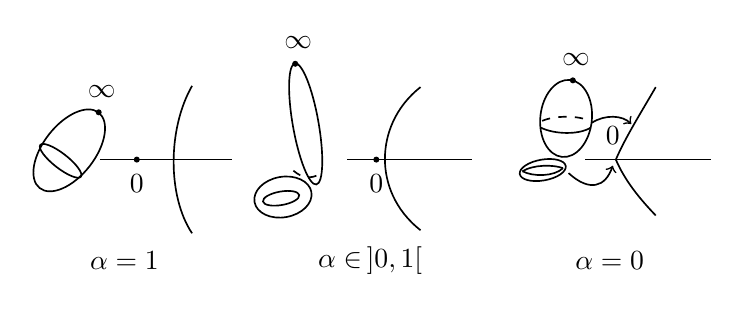
\begin{tikzpicture}[line width=0.6pt,scale=0.78]
  \begin{scope}[xshift=0cm]
    \draw (-0.05,0.2) -- (2.1,0.2);
    \fill (0.55,0.2) circle (1.4pt);
    \node[below] at (0.55,0.12) {$0$};
    \draw[rotate around={-38:(-0.55,0.35)}] (-0.55,0.35) ellipse (0.42 and 0.78);
    \draw[rotate around={-38:(-0.69,0.18)}] (-0.69,0.18) ellipse (0.42 and 0.12);
    \fill (-0.07,0.97) circle (1.4pt);
    \node[above] at (-0.02,1.05) {$\infty$};
    \draw (1.45,1.40) .. controls (1.05,0.70) and (1.05,-0.40) .. (1.45,-1.00);
    \node at (0.35,-1.45) {$\alpha=1$};
  \end{scope}
  \begin{scope}[xshift=3.9cm]
    \draw (0.08,0.2) -- (2.1,0.2);
    \fill (0.55,0.2) circle (1.4pt);
    \node[below] at (0.55,0.12) {$0$};
    \draw[rotate around={10:(-0.60,0.78)}] (-0.60,0.78) ellipse (0.21 and 1.00);
    \fill (-0.77,1.76) circle (1.4pt);
    \node[above] at (-0.72,1.84) {$\infty$};
    \draw[dashed] (-0.80,0.02) .. controls (-0.66,-0.10) and (-0.52,-0.12) .. (-0.38,-0.04);
    \draw[rotate around={10:(-0.97,-0.41)}] (-0.97,-0.41) ellipse (0.47 and 0.33);
    \draw[rotate around={10:(-1.00,-0.43)}] (-1.00,-0.43) ellipse (0.30 and 0.11);
    \draw (1.27,1.38) .. controls (0.85,1.05) and (0.69,0.60) .. (0.69,0.21)
      .. controls (0.69,-0.18) and (0.85,-0.62) .. (1.27,-0.95);
    \node at (0.45,-1.45) {$\alpha\in\,]0,1[$};
  \end{scope}
  \begin{scope}[xshift=7.8cm]
    \draw (0.05,0.2) -- (2.1,0.2);
    \node[above] at (0.50,0.28) {$0$};
    \draw[rotate around={-6:(-0.26,0.87)}] (-0.26,0.87) ellipse (0.42 and 0.63);
    \draw[dashed] (-0.65,0.83) .. controls (-0.45,0.92) and (-0.05,0.92) .. (0.12,0.83);
    \draw (-0.67,0.72) .. controls (-0.45,0.61) and (-0.05,0.60) .. (0.14,0.72);
    \fill (-0.15,1.49) circle (1.4pt);
    \node[above] at (-0.10,1.57) {$\infty$};
    \draw[rotate around={10:(-0.64,0.03)}] (-0.64,0.03) ellipse (0.38 and 0.17);
    \draw (-0.97,0.01) .. controls (-0.80,0.12) and (-0.46,0.12) .. (-0.31,0.06);
    \draw (-0.97,0.01) .. controls (-0.80,-0.08) and (-0.46,-0.08) .. (-0.31,0.06);
    \draw (1.20,1.38) .. controls (0.95,0.95) and (0.70,0.55) .. (0.55,0.20)
      .. controls (0.70,-0.15) and (0.95,-0.45) .. (1.20,-0.71);
    \draw[->] (0.16,0.80) .. controls (0.38,0.94) and (0.66,0.92) .. (0.80,0.78);
    \draw[->] (-0.22,-0.02) .. controls (0.12,-0.33) and (0.38,-0.25) .. (0.50,0.10);
    \node at (0.45,-1.45) {$\alpha=0$};
  \end{scope}
\end{tikzpicture}
\caption{}
\label{fig:cubic-limit-alpha}
\end{figure}

\begin{exercise}[整\trPeriodic\trForm]\label{ex:ch14-034-integral-periods}
设 $\alpha$ 是\trManifold{} $V$ 上的一个\trClosed{} 1-\trForm。假设 $\alpha$ 具有“整\trPeriodic”\footnote{意思是说，$\alpha$ 的\trRham{}\trCohomology{}类落在映射 $H^1(V;\ZZ)\to H^1(V;\RR)$ 的像之中。}，也就是说，按\cref{subsec:cover-closed-form}中的记号，$\varphi_\alpha$ 的\trImage{}包含在 $\ZZ\subset\RR$ 之中。证明：公式
\[
f(x)=\int_{x_0}^{x}\alpha
\]
定义了一个映射 $f\colon V\to\RR/\ZZ$，并且
\[
f^\star\,d\theta=2\pi\alpha\text{。}
\]

证明：\trIntegrationCover{} $\pi\colon\widetilde{V}\to V$ 是图
\[
\begin{tikzcd}
\widetilde{V}\ar[r,"\widetilde{f}"]\ar[d,"\pi"'] & \RR\ar[d,"\exp"]\\
V\ar[r,"f"'] & \RR/\ZZ
\end{tikzcd}
\]
（或\cref{fig:cover-helix}）中那个\trCovering{}的拉回，并且它是循环的。\footnote{译注：$\varphi_\alpha$ 的\trImage{}一般只是 $\ZZ$ 的子群 $d\ZZ$（$d\ge1$）；此时 $\exp\colon\RR\to\RR/\ZZ$ 沿 $f$ 的拉回共有 $d$ 个\trConnectedComponent（例如 $\alpha=0$ 时 $f$ 为常值，拉回即 $V\times\ZZ$，完全不\trConnected），其中单个\trConnectedComponent{}在 $V$ 上的覆叠才以 $\ZZ$ 为其\trCovering{}群。故所证者应取含指定的\trLift{}基点的那个\trConnectedComponent（或补设 $\varphi_\alpha$ 为\trSurjective）；此处照原书排印，存疑备案。——译者注}接着，在\trProjectiveSpace{} $\CP^n(\CC)$ 上考虑\trActionForm{} $\alpha_H$（如\cref{subsec:action-form}中那般）。验证：我们仍有
\[
\int_{S^2}w^\star\omega\in\ZZ\text{。}
\]
由此推出：$\scr{L}\CP^n(\CC)$ 存在一个无限循环\trCovering，使得 $\alpha_H$ 在其上具有一个原函数 $\widetilde{f}_H$。
\end{exercise}

\begin{figure}[htbp]
\centering
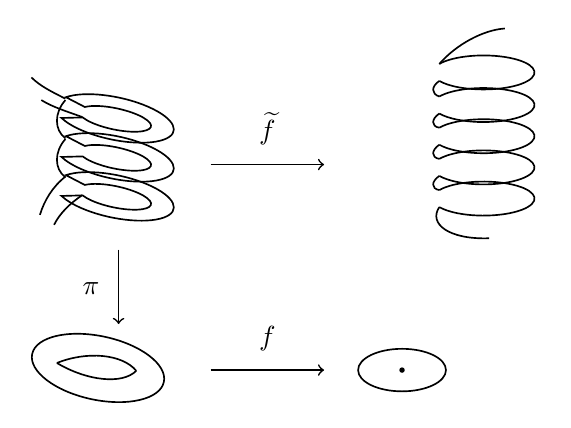
\begin{tikzpicture}[line width=0.6pt,scale=0.9]
  \begin{scope}[yshift=0cm]
    \begin{scope}[shift={(0,-0.10)},rotate around={-12:(0,0)}]
      \draw (-0.74,0.15) arc[start angle=150, end angle=-150, x radius=0.85, y radius=0.30]
        -- (-0.45,-0.08) arc[start angle=-150, end angle=150, x radius=0.52, y radius=0.15] -- cycle;
    \end{scope}
    \begin{scope}[shift={(0,-0.65)},rotate around={-12:(0,0)}]
      \draw (-0.74,0.15) arc[start angle=150, end angle=-150, x radius=0.85, y radius=0.30]
        -- (-0.45,-0.08) arc[start angle=-150, end angle=150, x radius=0.52, y radius=0.15] -- cycle;
    \end{scope}
    \begin{scope}[shift={(0,-1.20)},rotate around={-12:(0,0)}]
      \draw (-0.74,0.15) arc[start angle=150, end angle=-150, x radius=0.85, y radius=0.30]
        -- (-0.45,-0.08) arc[start angle=-150, end angle=150, x radius=0.52, y radius=0.15] -- cycle;
    \end{scope}
    \draw (-0.70,0.16) .. controls (-0.86,-0.02) and (-0.86,-0.26) .. (-0.70,-0.38);
    \draw (-0.70,-0.39) .. controls (-0.86,-0.57) and (-0.86,-0.81) .. (-0.70,-0.93);
    \draw (-0.70,0.18) .. controls (-0.90,0.28) and (-1.06,0.36) .. (-1.18,0.48);
    \draw (-0.46,-0.08) .. controls (-0.68,0.00) and (-0.88,0.06) .. (-1.04,0.16);
    \draw (-0.70,-0.92) .. controls (-0.88,-1.06) and (-1.00,-1.26) .. (-1.06,-1.46);
    \draw (-0.46,-1.18) .. controls (-0.64,-1.30) and (-0.78,-1.44) .. (-0.86,-1.60);
  \end{scope}
  \begin{scope}[xshift=5.2cm,yshift=0.25cm]
    \draw (0.30,0.92) .. controls (0.00,0.90) and (-0.38,0.70) .. (-0.624,0.42);
    \draw (-0.624,0.42) arc[start angle=150, end angle=-150, x radius=0.72, y radius=0.24];
    \draw (-0.624,0.18) .. controls (-0.74,0.10) and (-0.74,-0.00) .. (-0.624,-0.04);
    \draw (-0.624,-0.04) arc[start angle=150, end angle=-150, x radius=0.72, y radius=0.24];
    \draw (-0.624,-0.28) .. controls (-0.74,-0.36) and (-0.74,-0.46) .. (-0.624,-0.48);
    \draw (-0.624,-0.48) arc[start angle=150, end angle=-150, x radius=0.72, y radius=0.24];
    \draw (-0.624,-0.72) .. controls (-0.74,-0.80) and (-0.74,-0.90) .. (-0.624,-0.92);
    \draw (-0.624,-0.92) arc[start angle=150, end angle=-150, x radius=0.72, y radius=0.24];
    \draw (-0.624,-1.16) .. controls (-0.74,-1.24) and (-0.74,-1.34) .. (-0.624,-1.36);
    \draw (-0.624,-1.36) arc[start angle=150, end angle=-150, x radius=0.72, y radius=0.24];
    \draw (-0.624,-1.60) .. controls (-0.78,-1.83) and (-0.50,-2.06) .. (0.08,-2.04);
  \end{scope}
  \draw[->] (1.35,-0.75) -- (2.95,-0.75);
  \node[above] at (2.15,-0.62) {$\widetilde{f}$};
  \draw[->] (0.05,-1.95) -- (0.05,-3.00);
  \node[left] at (-0.08,-2.50) {$\pi$};
  \draw[rotate around={-12:(-0.24,-3.62)}] (-0.24,-3.62) ellipse (0.95 and 0.45);
  \draw (-0.82,-3.55) .. controls (-0.40,-3.38) and (0.10,-3.42) .. (0.30,-3.66);
  \draw (-0.82,-3.55) .. controls (-0.40,-3.80) and (0.10,-3.86) .. (0.30,-3.66);
  \draw[->] (1.35,-3.65) -- (2.95,-3.65);
  \node[above] at (2.15,-3.52) {$f$};
  \draw (4.05,-3.65) ellipse (0.62 and 0.30);
  \fill (4.05,-3.65) circle (1.1pt);
\end{tikzpicture}
\caption{}
\label{fig:cover-helix}
\end{figure}

